\documentclass[a0]{a0poster}
\usepackage{zhposter}

\sectionoutlineon  % comment out to hide outline before each section
\footlineon  % comment out to hide footline
% \frametitleleft  % comment out to center frame title
% \onelinebib  % uncomment to put bibliography entries in one line

\usepackage{tikz}
\usepackage{mathtools}

% commands
\newcommand{\ones}{{\bf 1{}}}  % vector with all components one
\newcommand{\reals}{{\bf R{}}}  % real numbers
\newcommand{\ints}{{\bf Z{}}}  % integers
\newcommand{\symms}{{\bf S{}}}  % symmetric matrices
\newcommand{\prob}{\mathop{\bf prob{}}}  % probability
\newcommand{\expect}{\mathop{\bf E{}}}  % expectation
\newcommand{\var}{\mathop{\bf var}}  % variance
\newcommand{\card}{\mathop{\bf card}}  % cardinality
\renewcommand{\dim}{\mathop{\bf dim}}  % dimension
\newcommand{\dom}{\mathop{\bf dom}}  % domain
\newcommand{\dist}{\mathop{\bf dist}}  % distance
\newcommand{\tr}{\mathop{\bf tr}}  % trace
\newcommand{\diag}{\mathop{\bf diag}}  % diagonal matrix
\newcommand{\rank}{\mathop{\bf rank}}  % rank
\newcommand{\argmax}{\mathop{\rm argmax}}  % argmax
\newcommand{\argmin}{\mathop{\rm argmin}}  % argmin
\newcommand{\supp}{\mathop{\bf supp}}  % support
\newcommand{\aff}{\mathop{\bf aff}}  % affine hull
\newcommand{\conv}{\mathop{\bf conv}}  % convex hull
\newcommand{\rg}{\mathop{\cal R{}}}  % range
\newcommand{\nl}{\mathop{\cal N{}}}  % null space
\newcommand{\itr}{\mathop{\bf int}}  % interior
\newcommand{\ri}{\mathop{\bf relint}}  % relative interior
\newcommand{\cl}{\mathop{\bf cl}}  % closure
\newcommand{\bd}{\mathop{\bf bd}}  % boundary
\newcommand{\epi}{\mathop{\bf epi}}  % epigraph
\newcommand{\norm}[1]{{\lVert #1 \rVert}}  % norm
\newcommand{\lambdamax}{{\lambda_{\rm max}}}  % max eigenvalue
\newcommand{\lambdamin}{{\lambda_{\rm min}}}  % min eigenvalue
\newcommand{\ball}{{\cal B{}}}  % ball

\newcommand{\cf}{{\rmfamily\itshape cf.}}
\newcommand{\eg}{{\rmfamily\itshape e.g.}}
\newcommand{\ie}{{\rmfamily\itshape i.e.}}
\newcommand{\etc}{{\rmfamily\itshape etc.}}
\newcommand{\etal}{{\rmfamily\itshape et al.}}

\usepackage{listings}
\usepackage{xcolor}

\definecolor{codegreen}{rgb}{0,0.6,0}
\definecolor{codegray}{rgb}{0.5,0.5,0.5}
\definecolor{codepurple}{rgb}{0.58,0,0.82}
\definecolor{backcolour}{rgb}{0.95,0.95,0.92}

\lstdefinestyle{zhstyle}{
    backgroundcolor=\color{backcolour},
    frame=leftline,
    % framerule=0.1pt,
    commentstyle=\color{codegreen},
    keywordstyle=\color{magenta},
    numberstyle=\small\color{codegray},
    stringstyle=\color{codepurple},
    basicstyle=\ttfamily\small,
    breakatwhitespace=false,
    breaklines=true,
    captionpos=b,
    keepspaces=true,
    numbers=left,
    numbersep=5pt,
    showspaces=false,
    showstringspaces=false,
    showtabs=false,
    tabsize=2
}
\lstset{style=zhstyle}

\lstdefinelanguage{zhpython}{%
    sensitive=true,%
    morekeywords={and, as, assert, break, class, continue, def, del, elif,%
        else, except, exec, finally, for, from, global, if, import, in, is,%
        lambda, not, or, pass, print, raise, return, try, while, with, yield},%
    morecomment=[l]\#,%
    morestring=[s]{'''}{'''},%
    morestring=[s]{"""}{"""},%
    morestring=[b]',%
    morestring=[b]"%
}

\begin{document}
\begin{textblock}{15}(0,0)
    \title{Multi-convex Programming for\\[0.1\baselineskip]Discrete Latent Factor Models Prototyping}
\end{textblock}

\begin{textblock}{15}(0,1.3)
    {\Large\bfseries Hao Zhu, Shengchao Yan, Jasper Hoffmann, and Joschka Boedecker}\\[0.5\baselineskip]
    {\Large\color{bluegray}\emph{IN-CODE Retreat, 2025}}
\end{textblock}

\begin{textblock}{3}(20,-0.2)
    \begin{center}
        
\includegraphics[height=10cm]{media/dlfm_github.pdf}\\
        {\footnotesize\texttt{https://github.com/nrgrp/dlfm}}
    \end{center}
\end{textblock}

\begin{textblock}{5}(15,-0.2)
    \begin{flushleft}
        
\includegraphics[height=1in]{media/nrlogo.pdf}
        \hspace*{1in}
        
\includegraphics[height=2in]{media/incode_logo.pdf}\\[1in]
        
\includegraphics[height=1in]{media/ufr_logo.pdf}
    \end{flushleft}
\end{textblock}

\begin{textblock}{7}(0,2)
    \hrule\vspace*{0.5\baselineskip}
    \begin{itemize}
        \item DLFMs appear in domains such as machine learning, economics, signal processing, control, \etc\
        \item in neuroscience and psychology, DLFMs provide interpretable characterizations of neural population activities and subject behavior
        \item currently, fitting a DLFM to some dataset relies on customized solver for individual models
            \begin{itemize}
                \item requires lots of background knowledge (both theoretical and technical) to implement
                \item limited to the targeted specific instance of DLFMs
                \item difficult to add regularization terms and constraints on the DLFM parameters and latent factors
            \end{itemize}
        \item we propose a framework for specifying and solving DLFM fitting problems
            \begin{itemize}
                \item supports DLFMs with loss functions and constraints of the fitting problem convex (even the fitting problem itself is not), including a wide range of regression and classification models
                \item allows the users to fit a DLFM to some dataset easily (within a couple of lines of code) in high level human readable language, close to the math
            \end{itemize}
    \end{itemize}
\end{textblock}

\begin{textblock}{7}(0,4.55)
    \hrule\vspace*{0.5\baselineskip}
    \Head{Discrete latent factor models (DLFMs)}

    DLFMs are generally expressed as
    \[
        z \sim \prob(z),\quad
        y \sim \prob(y \mid x, z, \theta)
    \]
    \begin{itemize}
        \item $z \in \{e_1, \ldots, e_K\} \subseteq \reals^K$ is the \emph{latent factor} (in vector form), $\theta$ is the \emph{model parameter}
        \item $x$ and $y$ are the \emph{feature} and \emph{observation}, respectively
    \end{itemize}
\end{textblock}

\begin{textblock}{7}(0,6.3)
    \hrule\vspace*{0.5\baselineskip}
    \Head{Standard DLFM fitting problems}

    \begin{equation}\label{prob:std_dlfm}
        \begin{array}{ll}
            \mbox{minimize} & \sum_{i = 1}^{m} z_i^T r_i = \sum_{i = 1}^{m} z_i^T (f(x_i, y_i; \theta_1), \ldots, f(x_i, y_i; \theta_K))\\
            \mbox{subject to} & z_i \in {\{0, 1\}}^K,\quad \card z_i = 1,\quad i = 1, \ldots, m\\
            & \theta_i \in \cvxset,\quad i = 1, \ldots, K
        \end{array}
    \end{equation}
    \begin{itemize}
        \item variables: model parameters $\theta_1, \ldots, \theta_K$ and latent factors $z_1, \ldots, z_m$
        \item data: feature-observation pairs ${\{x_i, y_i\}}_{i = 1}^m$
        \item the feasible set $\cvxset$ is closed and convex; the loss function $f$ is convex and resolves to scalar
    \end{itemize}
    \Subhead{Regression models}
        \[
            f(x, y; \theta) = g(x^T \theta - y)
        \]
        \begin{itemize}
            \item $x, \theta \in \reals^n$, $y \in \reals$, $g \colon \reals \to \reals$ is some loss function, \eg,
                \begin{itemize}
                    \item (squared) $\ell_p$-loss: $g(u) = u^2$, $g(u) = \norm{u}_p$ for $p \in [1, \infty]$
                    \item Huber loss: $f(u) = u^2$ for $|u| \leq \delta$, and $f(u) = 2 \delta |u| - \delta^2$ for $|u| > \delta$
                \end{itemize}
            \item nonscalar observations: $g(u) = \norm{u}_2^2$, $g(u) = \norm{u}_1$; $g(U) = \norm{U}_F^2 = \tr(U^T U)$
        \end{itemize}
    \Subhead{Classification models}
    \[
        f(X, y; \theta) = -\log\left(\frac{y^T \exp u}{\sum_{i = 1}^{p} \exp u_i}\right),\quad u = X \theta
    \]
    \begin{itemize}
        \item $X \in \reals^{p \times n}$, $y \in \{e_1, \ldots, e_p\} \subseteq \reals^p$, $\theta \in \reals^n$
        \item includes binary logistic regression as a special case
        \item readily adapted to deal with hinge loss or exponential loss
    \end{itemize}
    \Subhead{Constraints on model parameters}
    \begin{itemize}
        \item nonnegative orthant $\theta \succeq 0$, unit norm ball $\norm{\theta}_2 \leq 1$, probability simplex $\ones^T \theta = 1$
    \end{itemize}
\end{textblock}

\begin{textblock}{7}(8,2)
    \hrule\vspace*{0.5\baselineskip}
    \Head{Heuristic solution via BCD}

    relaxing the mixed integer constraints in (\ref{prob:std_dlfm}), we have
    \begin{equation}\label{prob:relax_dlfm}
        \begin{array}{ll}
            \mbox{minimize} & \sum_{i = 1}^{m} z_i^T r_i = \sum_{i = 1}^{m} z_i^T (f(x_i, y_i; \theta_1), \ldots, f(x_i, y_i; \theta_K))\\
            \mbox{subject to} & 0 \preceq z_i \preceq \ones,\quad \ones^T z_i = 1,\quad i = 1, \ldots, m\\
            & \theta_i \in \cvxset,\quad i = 1, \ldots, K
        \end{array}
    \end{equation}
    to solve the multi-convex problem (\ref{prob:relax_dlfm}), in each block coordinate descent (BCD) iteration, we alternate between solving the problems
    \[
        \mbox{(P)}\quad
        \begin{array}{ll}
            \mbox{minimize} & \sum_{i = 1}^{m} \tilde{z}_i^T r_i\\
            \mbox{subject to} & r_i = {(f(x_i, y_i; \theta_k))}_{k = 1}^K,\quad \theta_k \in \cvxset\\
            & i = 1, \ldots, m,\quad k = 1, \ldots, K\\
        \end{array}\qquad
        \mbox{(F)}\quad
        \begin{array}{ll}
            \mbox{minimize} & \sum_{i = 1}^{m} z_i^T \tilde{r}_i\\
            \mbox{subject to} & 0 \preceq z_i \preceq \ones,\quad \ones^T z_i = 1\\
            & i = 1, \ldots, m
        \end{array}
    \]
    \begin{itemize}
        \item P-problem has variables: $\theta_1, \ldots, \theta_K$ and data ${\{x_i, y_i\}}_{i = 1}^m$ from the dataset, $\tilde{z}_1, \ldots, \tilde{z}_m \in \reals^K$ corresponding to the optimal point of the F-problem in the last iteration
        \item F-problem has variables: $z_1, \ldots, z_m \in \reals^K$ and data $\tilde{r}_i = (f(x_i, y_i; \tilde{\theta}_1), \ldots, f(x_i, y_i; \tilde{\theta}_K))$, $i = 1, \ldots, m$, where $\tilde{\theta}_1, \ldots, \tilde{\theta}_K$ are the optimal point of the P-problem in the last iteration
    \end{itemize}

    \Subhead{Regularizations}
    \begin{itemize}
        \item for sparse model parameters $\theta_1, \ldots, \theta_K$: $\lambda \sum_{k = 1}^{K} \norm{\theta_k}_1$ with $\lambda \geq 0$
        \item for sparse latent factor change: $\lambda \sum_{i = 1}^{m - 1} \Dkl(z_i, z_{i + 1})$ with $\lambda \geq 0$ ($\Dkl$ is the KL-divergence)
    \end{itemize}
\end{textblock}

\begin{textblock}{7}(8,6.55)
    \hrule\vspace*{0.5\baselineskip}
    \Head{Implementation}
    \Subhead{Specifying a problem}
    (only the commented lines need to be specified by the user)
    \lstinputlisting[language=zhpython]{media/specify_prob.py}

    \Subhead{Running BCD iterations}
    (quit when the optimal values of the P- and F-problem converge)
    \lstinputlisting[language=zhpython]{media/bcd_iter.py}
\end{textblock}

\begin{textblock}{7}(16,2)
\hrule\vspace*{0.5\baselineskip}
\Head{Examples}
\Subhead{Hierarchical forgetting Q-learning}
consider an agent performing a $p$-armed bandit:
\begin{itemize}
    \item reward signal $u(t) \in \{0\} \cup \{e_1, \ldots, e_p\} \subseteq \reals^p$ indicates if the action at time $t - 1$ is rewarded
    \item action at time $t$ is selected under parameters $\theta(t) \in \{\theta_1, \ldots, \theta_K\} \subseteq \reals^n$, according to
        \[
            \begin{aligned}
                &v(t) = X(t) \theta(t),\quad
                X(t) = \left[
                    \begin{array}{cccc}
                        u(t) & u(t - 1) & \cdots & u(t - n + 1)
                    \end{array}
                \right] \in \reals^{p \times n},\\
                &y(t) \sim {\rm Cat}(\{e_1, \ldots, e_p\},\ \exp v(t) / \ones^T \exp v(t))
            \end{aligned}
        \]
\end{itemize}
the optimization problems in each BCD iterations are
\[
    \begin{aligned}
        &\mbox{(P)}\quad
        \begin{array}{ll}
            \mbox{minimize} & \sum_{t = 1}^{m} {\tilde{z}(t)}^T r(t)\\
            \mbox{subject to} & r(t) = -\log \left(\frac{{y(t)}^T \exp(X(t)\theta_1)}{\ones^T \exp(X(t)\theta_1)},\ \frac{{y(t)}^T \exp(X(t)\theta_2)}{\ones^T \exp(X(t)\theta_2)}\right),\quad t = 1, \ldots, m\\
            & \theta_1 \geq 0,\quad \theta_{1, 1} \geq \cdots \geq \theta_{1, 5},\quad \theta_2 \leq 0,\quad \theta_{2, 1} \leq \cdots \leq \theta_{2, 5}
        \end{array}\\[5pt]
        &\mbox{(F)}\quad
        \begin{array}{ll}
            \mbox{minimize} & \sum_{t = 1}^{m} {z(t)}^T \tilde{r}(t) + \lambda \sum_{t = 1}^{m - 1} \Dkl(z(t), z(t + 1))\\
            \mbox{subject to} & 0 \preceq z(t) \preceq \ones,\quad \ones^T z(t) = 1,\quad t = 1, \ldots, m
        \end{array}
    \end{aligned}
\]
\begin{figure}
    \centering
    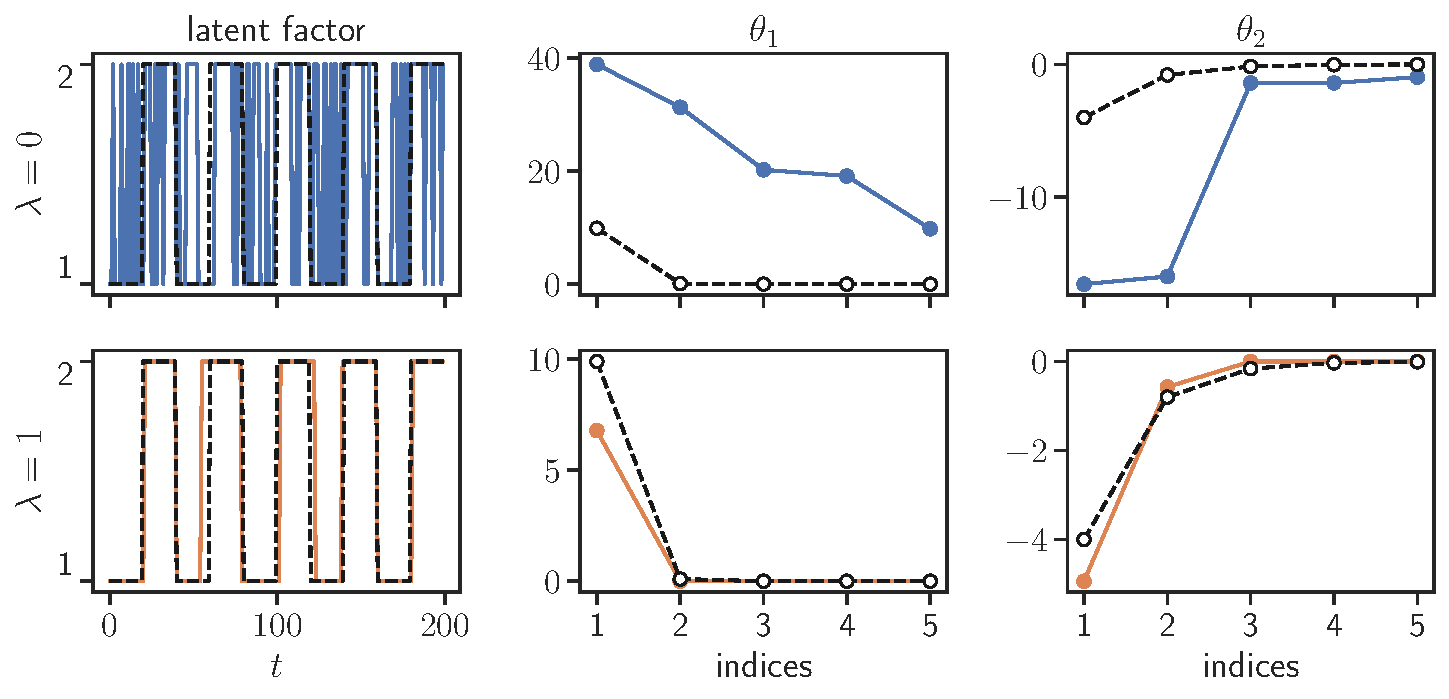
\includegraphics[width=0.8\textwidth]{media/hier_forget_q_learning.pdf}
    \caption{\small
        Colored solid lines: recovered latent factors and model parameters.
        Black dashed lines: ground truth.
    }
\end{figure}

\Subhead{Input-output hidden Markov model}
consider a dataset generated according to
\begin{itemize}
    \item $\hat{z}(t) \in \{1, \ldots, K\}$ from a $K$-state Markov chain, with coefficients $\theta_{\hat{z}(t)} \in \{\theta_1, \ldots, \theta_K\} \subseteq \reals^n$
    \item $y(t) \in \{0, 1\}$ with $\prob(y(t) = 1) = 1/(1 + \exp(-{x(t)}^T \theta_{\hat{z}(t)}))$, given feature vector $x(t) \in \reals^n$
\end{itemize}
\begin{minipage}{0.7\textwidth}
the optimization problems in each BCD iterations are
\[
    \begin{aligned}
        &\mbox{(P)}\quad
        \begin{array}{ll}
            \mbox{minimize} & \sum_{t = 1}^{m} {\tilde{z}(t)}^T r(t) + \lambda_\theta \sum_{k = 1}^{3} \norm{\theta_k}_2\\
            \mbox{subject to} & r(t) = -{\left(y(t){x(t)}^T \theta_k - \log\left(1 + e^{{x(t)}^T \theta_k}\right)\right)}_{k = 1}^{3}\\
            & \theta_{1, 1} \leq 0,\quad \theta_{2, 1} \geq 0,\quad \theta_{3, 1} \geq 0\\
            & t = 1, \ldots, m
        \end{array}\\[5pt]
        &\mbox{(F)}\quad
        \begin{array}{ll}
            \mbox{minimize} & \sum_{t = 1}^{m} {z(t)}^T \tilde{r}(t) + \lambda_z \sum_{t = 1}^{m - 1} \Dkl(z(t), z(t + 1))\\
            \mbox{subject to} & 0 \preceq z(t) \preceq \ones,\quad \ones^T z(t) = 1,\quad t = 1, \ldots, m
        \end{array}
    \end{aligned}
\]
\end{minipage}%
\begin{minipage}{0.3\textwidth}
    \begin{figure}
        \centering
        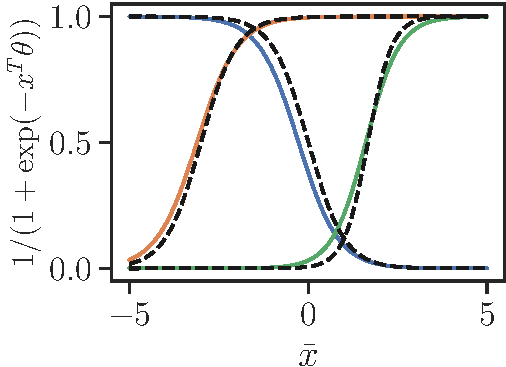
\includegraphics[width=\textwidth]{media/io_hmm_crop.eps}
        \caption{\small
            Colored solid lines: recovered decision curve.
            Black dashed lines: ground truth.
        }
    \end{figure}
\end{minipage}
\end{textblock}

\begin{textblock}{7}(16,11.2)
    \small
    \nocite{*}
    \bibliography{refs}
\end{textblock}

\end{document}